\documentclass{standalone}
\usepackage{pgfplots}
\pgfplotsset{compat=1.18}
\begin{document}

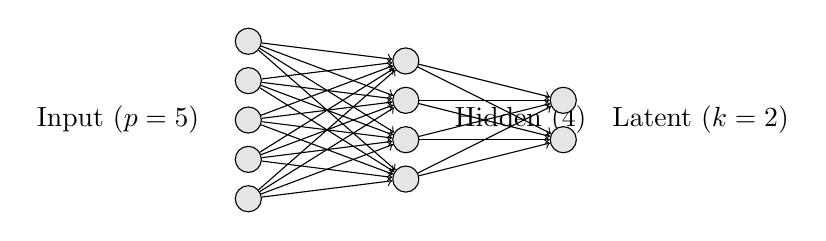
\begin{tikzpicture}
    \node[circle, draw, fill=gray!20] (i1) at (0, 0) {};
    \node[circle, draw, fill=gray!20] (i2) at (0, 0.5) {};
    \node[circle, draw, fill=gray!20] (i3) at (0, 1) {};
    \node[circle, draw, fill=gray!20] (i4) at (0, 1.5) {};
    \node[circle, draw, fill=gray!20] (i5) at (0, 2) {};
    \node[left] at (-0.5, 1) {Input ($p=5$)};
    
    \node[circle, draw, fill=gray!20] (h1) at (2, 0.25) {};
    \node[circle, draw, fill=gray!20] (h2) at (2, 0.75) {};
    \node[circle, draw, fill=gray!20] (h3) at (2, 1.25) {};
    \node[circle, draw, fill=gray!20] (h4) at (2, 1.75) {};
    \node[right] at (2.5, 1) {Hidden (4)};
    
    \node[circle, draw, fill=gray!20] (z1) at (4, 0.75) {};
    \node[circle, draw, fill=gray!20] (z2) at (4, 1.25) {};
    \node[right] at (4.5, 1) {Latent ($k=2$)};
    
    \foreach \i in {1,...,5}
        \foreach \j in {1,...,4}
            \draw[->] (i\i) -- (h\j);
    \foreach \i in {1,...,4}
        \foreach \j in {1,...,2}
            \draw[->] (h\i) -- (z\j);
\end{tikzpicture}
    \end{tikzpicture}

    \end{document}